\documentclass[twoside]{book}

% Packages required by doxygen
\usepackage{fixltx2e}
\usepackage{calc}
\usepackage{doxygen}
\usepackage[export]{adjustbox} % also loads graphicx
\usepackage{graphicx}
\usepackage[utf8]{inputenc}
\usepackage{makeidx}
\usepackage{multicol}
\usepackage{multirow}
\PassOptionsToPackage{warn}{textcomp}
\usepackage{textcomp}
\usepackage[nointegrals]{wasysym}
\usepackage[table]{xcolor}

% Font selection
\usepackage[T1]{fontenc}
\usepackage[scaled=.90]{helvet}
\usepackage{courier}
\usepackage{amssymb}
\usepackage{sectsty}
\renewcommand{\familydefault}{\sfdefault}
\allsectionsfont{%
  \fontseries{bc}\selectfont%
  \color{darkgray}%
}
\renewcommand{\DoxyLabelFont}{%
  \fontseries{bc}\selectfont%
  \color{darkgray}%
}
\newcommand{\+}{\discretionary{\mbox{\scriptsize$\hookleftarrow$}}{}{}}

% Page & text layout
\usepackage{geometry}
\geometry{%
  a4paper,%
  top=2.5cm,%
  bottom=2.5cm,%
  left=2.5cm,%
  right=2.5cm%
}
\tolerance=750
\hfuzz=15pt
\hbadness=750
\setlength{\emergencystretch}{15pt}
\setlength{\parindent}{0cm}
\setlength{\parskip}{0.2cm}
\makeatletter
\renewcommand{\paragraph}{%
  \@startsection{paragraph}{4}{0ex}{-1.0ex}{1.0ex}{%
    \normalfont\normalsize\bfseries\SS@parafont%
  }%
}
\renewcommand{\subparagraph}{%
  \@startsection{subparagraph}{5}{0ex}{-1.0ex}{1.0ex}{%
    \normalfont\normalsize\bfseries\SS@subparafont%
  }%
}
\makeatother

% Headers & footers
\usepackage{fancyhdr}
\pagestyle{fancyplain}
\fancyhead[LE]{\fancyplain{}{\bfseries\thepage}}
\fancyhead[CE]{\fancyplain{}{}}
\fancyhead[RE]{\fancyplain{}{\bfseries\leftmark}}
\fancyhead[LO]{\fancyplain{}{\bfseries\rightmark}}
\fancyhead[CO]{\fancyplain{}{}}
\fancyhead[RO]{\fancyplain{}{\bfseries\thepage}}
\fancyfoot[LE]{\fancyplain{}{}}
\fancyfoot[CE]{\fancyplain{}{}}
\fancyfoot[RE]{\fancyplain{}{\bfseries\scriptsize Generated on Wed Jun 10 2015 09\+:57\+:59 for My Project by Doxygen }}
\fancyfoot[LO]{\fancyplain{}{\bfseries\scriptsize Generated on Wed Jun 10 2015 09\+:57\+:59 for My Project by Doxygen }}
\fancyfoot[CO]{\fancyplain{}{}}
\fancyfoot[RO]{\fancyplain{}{}}
\renewcommand{\footrulewidth}{0.4pt}
\renewcommand{\chaptermark}[1]{%
  \markboth{#1}{}%
}
\renewcommand{\sectionmark}[1]{%
  \markright{\thesection\ #1}%
}

% Indices & bibliography
\usepackage{natbib}
\usepackage[titles]{tocloft}
\setcounter{tocdepth}{3}
\setcounter{secnumdepth}{5}
\makeindex

% Hyperlinks (required, but should be loaded last)
\usepackage{ifpdf}
\ifpdf
  \usepackage[pdftex,pagebackref=true]{hyperref}
\else
  \usepackage[ps2pdf,pagebackref=true]{hyperref}
\fi
\hypersetup{%
  colorlinks=true,%
  linkcolor=blue,%
  citecolor=blue,%
  unicode%
}

% Custom commands
\newcommand{\clearemptydoublepage}{%
  \newpage{\pagestyle{empty}\cleardoublepage}%
}


%===== C O N T E N T S =====

\begin{document}

% Titlepage & ToC
\hypersetup{pageanchor=false,
             bookmarks=true,
             bookmarksnumbered=true,
             pdfencoding=unicode
            }
\pagenumbering{roman}
\begin{titlepage}
\vspace*{7cm}
\begin{center}%
{\Large My Project }\\
\vspace*{1cm}
{\large Generated by Doxygen 1.8.9.1}\\
\vspace*{0.5cm}
{\small Wed Jun 10 2015 09:57:59}\\
\end{center}
\end{titlepage}
\clearemptydoublepage
\tableofcontents
\clearemptydoublepage
\pagenumbering{arabic}
\hypersetup{pageanchor=true}

%--- Begin generated contents ---
\chapter{Hierarchical Index}
\section{Jerarquía de la clase}
Esta lista de herencias esta ordenada aproximadamente por orden alfabético\+:\begin{DoxyCompactList}
\item Q\+Main\+Window\begin{DoxyCompactList}
\item \contentsline{section}{Drawing\+Window}{\pageref{class_drawing_window}}{}
\end{DoxyCompactList}
\item Q\+Widget\begin{DoxyCompactList}
\item \contentsline{section}{Line}{\pageref{class_line}}{}
\item \contentsline{section}{Tessellation}{\pageref{class_tessellation}}{}
\end{DoxyCompactList}
\end{DoxyCompactList}

\chapter{Class Index}
\section{Class List}
Here are the classes, structs, unions and interfaces with brief descriptions\+:\begin{DoxyCompactList}
\item\contentsline{section}{\hyperlink{class_drawing_window}{Drawing\+Window} }{\pageref{class_drawing_window}}{}
\item\contentsline{section}{\hyperlink{class_line}{Line} }{\pageref{class_line}}{}
\item\contentsline{section}{\hyperlink{class_tessellation}{Tessellation} }{\pageref{class_tessellation}}{}
\end{DoxyCompactList}

\chapter{Class Documentation}
\hypertarget{class_drawing_window}{}\section{Drawing\+Window Class Reference}
\label{class_drawing_window}\index{Drawing\+Window@{Drawing\+Window}}


{\ttfamily \#include $<$drawing\+Window.\+h$>$}

Inheritance diagram for Drawing\+Window\+:\begin{figure}[H]
\begin{center}
\leavevmode
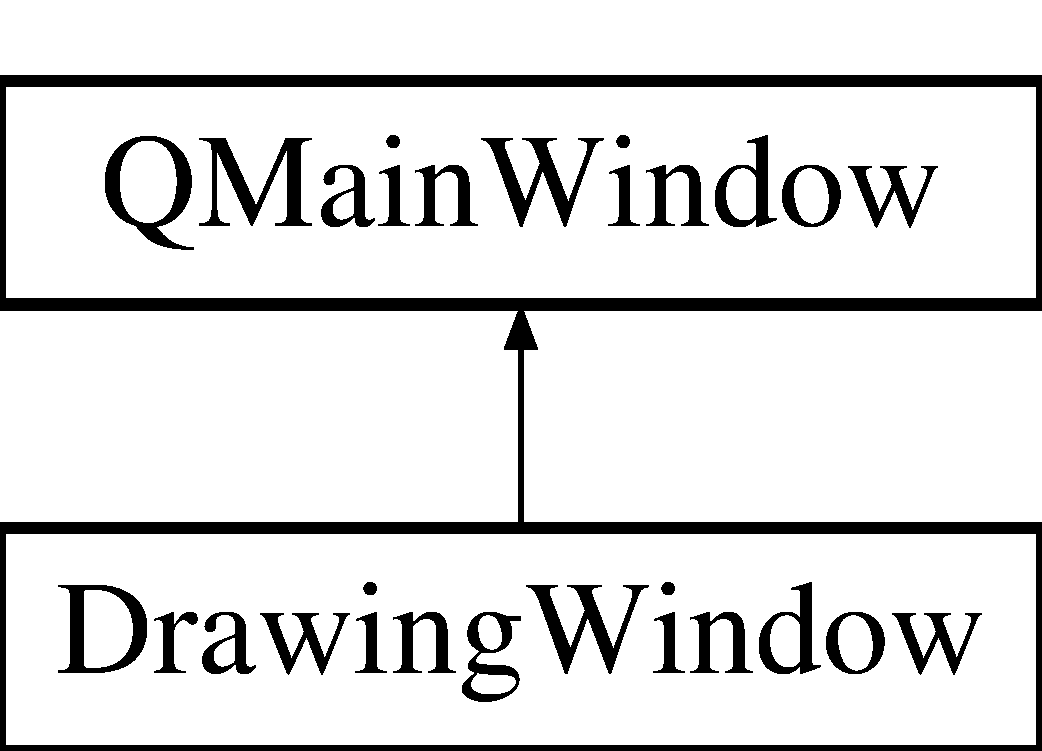
\includegraphics[height=2.000000cm]{class_drawing_window}
\end{center}
\end{figure}
\subsection*{Public Member Functions}
\begin{DoxyCompactItemize}
\item 
\hypertarget{class_drawing_window_aff3d1b3cbeee8f0e92b49c050d8ca494}{}\hyperlink{class_drawing_window_aff3d1b3cbeee8f0e92b49c050d8ca494}{Drawing\+Window} (Q\+Widget $\ast$parent=0)\label{class_drawing_window_aff3d1b3cbeee8f0e92b49c050d8ca494}

\begin{DoxyCompactList}\small\item\em Constructor. \end{DoxyCompactList}\item 
\hypertarget{class_drawing_window_a0d07890a752adffee1f92a463561dcb6}{}\hyperlink{class_drawing_window_a0d07890a752adffee1f92a463561dcb6}{$\sim$\+Drawing\+Window} ()\label{class_drawing_window_a0d07890a752adffee1f92a463561dcb6}

\begin{DoxyCompactList}\small\item\em Destructor. \end{DoxyCompactList}\item 
void \hyperlink{class_drawing_window_ac5a412fbb239f1f57cabe7a850e1e4fb}{add\+Tessellation} (\hyperlink{class_tessellation}{Tessellation} \&t)
\begin{DoxyCompactList}\small\item\em Add a tessalation to the window. \end{DoxyCompactList}\item 
void \hyperlink{class_drawing_window_a3097e096223530c9f93737441d77422f}{add\+Line} (int x0, int y0, int x1, int y1, int width, Q\+Color color)
\begin{DoxyCompactList}\small\item\em Add a line to the window, specifying coordinates of the starting and end points. \end{DoxyCompactList}\item 
void \hyperlink{class_drawing_window_ae03504caa7648347ec56eb58cf5b5db4}{add\+Line\+Polar} (int x0, int y0, int length, double angle, int width, Q\+Color color)
\begin{DoxyCompactList}\small\item\em Add a line to the window, specifying coordinates of the starting point, the length and angle. \end{DoxyCompactList}\end{DoxyCompactItemize}
\subsection*{Protected Member Functions}
\begin{DoxyCompactItemize}
\item 
\hypertarget{class_drawing_window_aceb9c5cc4f2ef40d99aca7d3fbd4e91a}{}void \hyperlink{class_drawing_window_aceb9c5cc4f2ef40d99aca7d3fbd4e91a}{paint\+Event} (Q\+Paint\+Event $\ast$)\label{class_drawing_window_aceb9c5cc4f2ef40d99aca7d3fbd4e91a}

\begin{DoxyCompactList}\small\item\em Paints event. \end{DoxyCompactList}\end{DoxyCompactItemize}
\subsection*{Private Attributes}
\begin{DoxyCompactItemize}
\item 
\hypertarget{class_drawing_window_ad58ced401c1eaf6cfaf67a0f8f94ce18}{}Ui\+::\+Drawing\+Window $\ast$ {\bfseries ui}\label{class_drawing_window_ad58ced401c1eaf6cfaf67a0f8f94ce18}

\item 
vector$<$ \hyperlink{class_tessellation}{Tessellation} $\ast$ $>$ $\ast$ \hyperlink{class_drawing_window_a00c917f0910ac7b70729d6a48f0602ac}{v\+T}
\item 
vector$<$ \hyperlink{class_tessellation}{Tessellation} $\ast$ $>$ $\ast$ \hyperlink{class_drawing_window_a82bd46efc8a35b62fcd207c42aa49ade}{my\+Tessellation}
\item 
vector$<$ \hyperlink{class_line}{Line} $\ast$ $>$ $\ast$ \hyperlink{class_drawing_window_a6e1effc34bb2f2c43becfd1df203b693}{v\+L}
\end{DoxyCompactItemize}


\subsection{Detailed Description}
A class to create a drawing window to draw tessellations. 

\subsection{Member Function Documentation}
\hypertarget{class_drawing_window_a3097e096223530c9f93737441d77422f}{}\index{Drawing\+Window@{Drawing\+Window}!add\+Line@{add\+Line}}
\index{add\+Line@{add\+Line}!Drawing\+Window@{Drawing\+Window}}
\subsubsection[{add\+Line}]{\setlength{\rightskip}{0pt plus 5cm}void Drawing\+Window\+::add\+Line (
\begin{DoxyParamCaption}
\item[{int}]{x0, }
\item[{int}]{y0, }
\item[{int}]{x1, }
\item[{int}]{y1, }
\item[{int}]{width, }
\item[{Q\+Color}]{color}
\end{DoxyParamCaption}
)}\label{class_drawing_window_a3097e096223530c9f93737441d77422f}


Add a line to the window, specifying coordinates of the starting and end points. 


\begin{DoxyParams}{Parameters}
{\em x0} & starting coordinate x \\
\hline
{\em y0} & starting coordinate y \\
\hline
{\em x1} & end coordinate x \\
\hline
{\em y1} & end coordinate y \\
\hline
{\em width} & line width \\
\hline
{\em color} & line color \\
\hline
\end{DoxyParams}
\hypertarget{class_drawing_window_ae03504caa7648347ec56eb58cf5b5db4}{}\index{Drawing\+Window@{Drawing\+Window}!add\+Line\+Polar@{add\+Line\+Polar}}
\index{add\+Line\+Polar@{add\+Line\+Polar}!Drawing\+Window@{Drawing\+Window}}
\subsubsection[{add\+Line\+Polar}]{\setlength{\rightskip}{0pt plus 5cm}void Drawing\+Window\+::add\+Line\+Polar (
\begin{DoxyParamCaption}
\item[{int}]{x0, }
\item[{int}]{y0, }
\item[{int}]{length, }
\item[{double}]{angle, }
\item[{int}]{width, }
\item[{Q\+Color}]{color}
\end{DoxyParamCaption}
)}\label{class_drawing_window_ae03504caa7648347ec56eb58cf5b5db4}


Add a line to the window, specifying coordinates of the starting point, the length and angle. 


\begin{DoxyParams}{Parameters}
{\em x0} & starting coordinate x \\
\hline
{\em y0} & starting coordinate y \\
\hline
{\em length} & -\/ length of the line \\
\hline
{\em angle} & -\/ angle of the line \\
\hline
{\em width} & -\/ line width \\
\hline
{\em color} & -\/ line color \\
\hline
\end{DoxyParams}
\hypertarget{class_drawing_window_ac5a412fbb239f1f57cabe7a850e1e4fb}{}\index{Drawing\+Window@{Drawing\+Window}!add\+Tessellation@{add\+Tessellation}}
\index{add\+Tessellation@{add\+Tessellation}!Drawing\+Window@{Drawing\+Window}}
\subsubsection[{add\+Tessellation}]{\setlength{\rightskip}{0pt plus 5cm}void Drawing\+Window\+::add\+Tessellation (
\begin{DoxyParamCaption}
\item[{{\bf Tessellation} \&}]{t}
\end{DoxyParamCaption}
)}\label{class_drawing_window_ac5a412fbb239f1f57cabe7a850e1e4fb}


Add a tessalation to the window. 


\begin{DoxyParams}{Parameters}
{\em t} & a tessellation object \\
\hline
\end{DoxyParams}


\subsection{Member Data Documentation}
\hypertarget{class_drawing_window_a82bd46efc8a35b62fcd207c42aa49ade}{}\index{Drawing\+Window@{Drawing\+Window}!my\+Tessellation@{my\+Tessellation}}
\index{my\+Tessellation@{my\+Tessellation}!Drawing\+Window@{Drawing\+Window}}
\subsubsection[{my\+Tessellation}]{\setlength{\rightskip}{0pt plus 5cm}vector$<${\bf Tessellation} $\ast$$>$$\ast$ Drawing\+Window\+::my\+Tessellation\hspace{0.3cm}{\ttfamily [private]}}\label{class_drawing_window_a82bd46efc8a35b62fcd207c42aa49ade}
vector of tesselation / vector de mosaicos \hypertarget{class_drawing_window_a6e1effc34bb2f2c43becfd1df203b693}{}\index{Drawing\+Window@{Drawing\+Window}!v\+L@{v\+L}}
\index{v\+L@{v\+L}!Drawing\+Window@{Drawing\+Window}}
\subsubsection[{v\+L}]{\setlength{\rightskip}{0pt plus 5cm}vector$<${\bf Line} $\ast$$>$$\ast$ Drawing\+Window\+::v\+L\hspace{0.3cm}{\ttfamily [private]}}\label{class_drawing_window_a6e1effc34bb2f2c43becfd1df203b693}
vector of line / vector de lineas \hypertarget{class_drawing_window_a00c917f0910ac7b70729d6a48f0602ac}{}\index{Drawing\+Window@{Drawing\+Window}!v\+T@{v\+T}}
\index{v\+T@{v\+T}!Drawing\+Window@{Drawing\+Window}}
\subsubsection[{v\+T}]{\setlength{\rightskip}{0pt plus 5cm}vector$<${\bf Tessellation}$\ast$ $>$$\ast$ Drawing\+Window\+::v\+T\hspace{0.3cm}{\ttfamily [private]}}\label{class_drawing_window_a00c917f0910ac7b70729d6a48f0602ac}
vector of tesselation / vector de mosaicos 

The documentation for this class was generated from the following files\+:\begin{DoxyCompactItemize}
\item 
drawing\+Window.\+h\item 
drawing\+Window.\+cpp\end{DoxyCompactItemize}

\hypertarget{class_line}{}\section{Referencia de la Clase Line}
\label{class_line}\index{Line@{Line}}


{\ttfamily \#include $<$line.\+h$>$}

Diagrama de herencias de Line\begin{figure}[H]
\begin{center}
\leavevmode
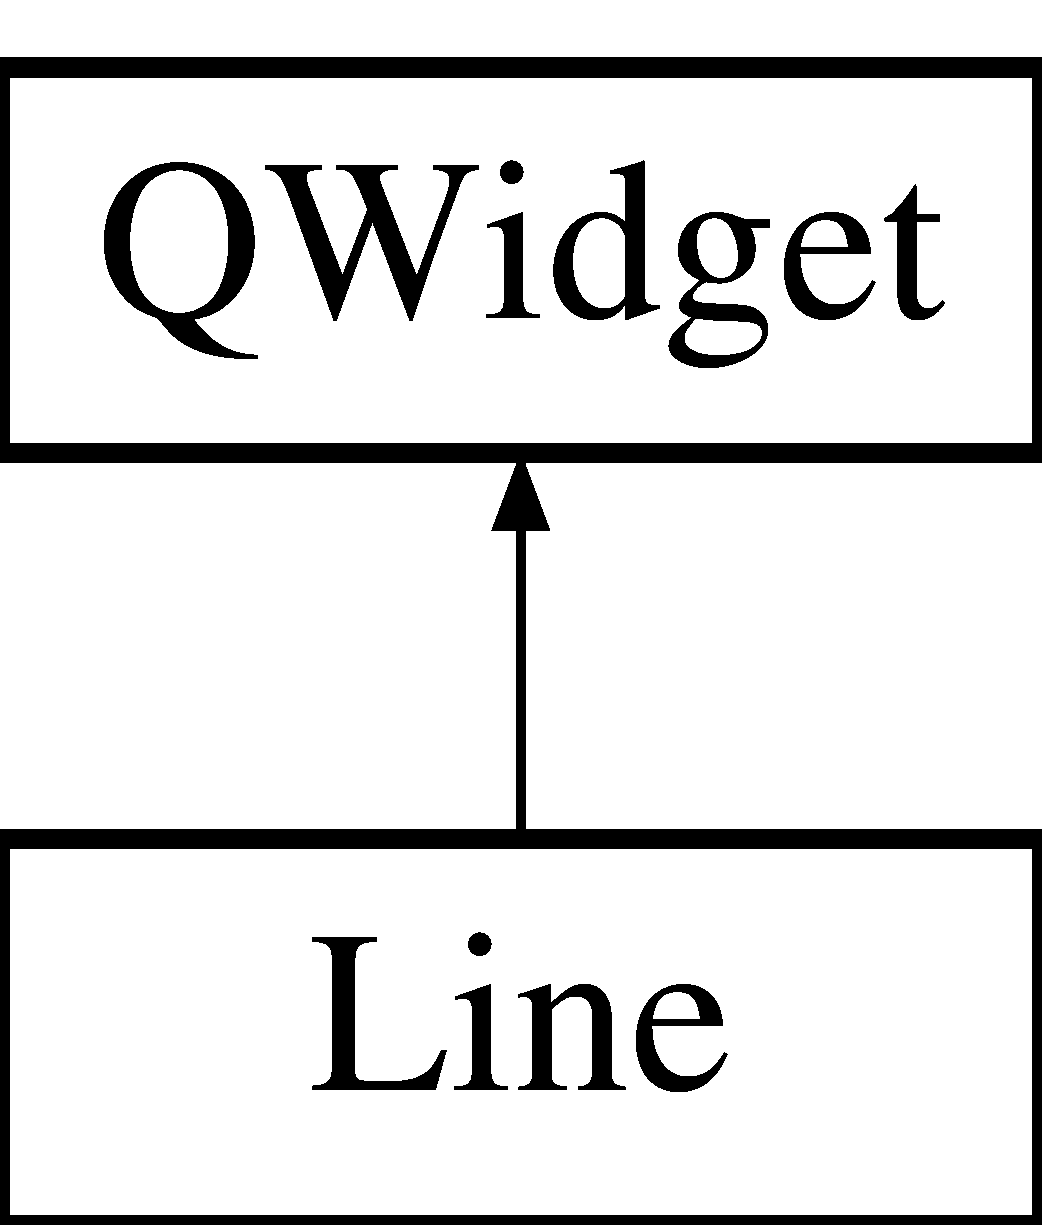
\includegraphics[height=2.000000cm]{class_line}
\end{center}
\end{figure}
\subsection*{Métodos públicos}
\begin{DoxyCompactItemize}
\item 
\hypertarget{class_line_a4d475f9d634f50933ca84e25d7cf32f9}{}\hyperlink{class_line_a4d475f9d634f50933ca84e25d7cf32f9}{Line} (Q\+Widget $\ast$parent=0)\label{class_line_a4d475f9d634f50933ca84e25d7cf32f9}

\begin{DoxyCompactList}\small\item\em Constructor que ajusta las coordenadas a 0, el color y el ancho del boligrafo a negro y 1 respectivamente. \end{DoxyCompactList}\item 
\hyperlink{class_line_a37f70dab8d5cc7560e6362093a3aa1b9}{Line} (int from\+X, int from\+Y, int to\+X, int to\+Y, int w, Q\+Color c, Q\+Widget $\ast$parent=0)
\begin{DoxyCompactList}\small\item\em Constructor de una linea, especificando las coordenadas (from\+X,from\+Y) y (to\+X,to\+Y) \end{DoxyCompactList}\item 
\hyperlink{class_line_a742b2aea487313953635d1e504c6b866}{Line} (int from\+X, int from\+Y, int length, double angle, int w, Q\+Color c, Q\+Widget $\ast$parent=0)
\begin{DoxyCompactList}\small\item\em Constructor de una linea, especificando la coordenada (from\+X, from\+Y) and el largo (length) y el angulo (angle). \end{DoxyCompactList}\item 
void \hyperlink{class_line_ac1475ffee823a7c05b2ac91bfe61596d}{set\+Coords} (int from\+X, int from\+Y, int to\+X, int to\+Y)
\begin{DoxyCompactList}\small\item\em Ajustador de las coordenadas de la linea. \end{DoxyCompactList}\item 
void \hyperlink{class_line_ac5b6d8e786cf3820fa36b8bda7130823}{setpen\+Color} (Q\+Color c)
\begin{DoxyCompactList}\small\item\em Ajustador del color del boligrafo. \end{DoxyCompactList}\item 
void \hyperlink{class_line_a346d88820371b5a4710eed8a638fc451}{set\+Pen\+Width} (int w)
\begin{DoxyCompactList}\small\item\em Ajustador del ancho del boligrafo. \end{DoxyCompactList}\item 
int \hyperlink{class_line_a0e23ee7edc154bd73fefab4d88cae150}{get\+X0} ()
\begin{DoxyCompactList}\small\item\em Devuelve la coordenada inicial x. \end{DoxyCompactList}\item 
int \hyperlink{class_line_a971146fd8bbf711123f03e45daf923c9}{get\+Y0} ()
\begin{DoxyCompactList}\small\item\em Devuelve la coordenada inicial y. \end{DoxyCompactList}\item 
int \hyperlink{class_line_a1f51d8df03219f5f63d656bc0e9b2830}{get\+X1} ()
\begin{DoxyCompactList}\small\item\em Devuelve la coordenada final x. \end{DoxyCompactList}\item 
int \hyperlink{class_line_a9cc398fdcf93212a3e4db28ac26a88a9}{get\+Y1} ()
\begin{DoxyCompactList}\small\item\em Devuelve la coordenada final y. \end{DoxyCompactList}\end{DoxyCompactItemize}
\subsection*{Métodos protegidos}
\begin{DoxyCompactItemize}
\item 
\hypertarget{class_line_a7e1f30fa9d7375fd67a2b4cf5a1b6a76}{}void \hyperlink{class_line_a7e1f30fa9d7375fd67a2b4cf5a1b6a76}{paint\+Event} (Q\+Paint\+Event $\ast$)\label{class_line_a7e1f30fa9d7375fd67a2b4cf5a1b6a76}

\begin{DoxyCompactList}\small\item\em La funcion para el evento de pintar es invocada automaticamente cada ves que evento de repintar ocurre. \end{DoxyCompactList}\end{DoxyCompactItemize}
\subsection*{Atributos privados}
\begin{DoxyCompactItemize}
\item 
int \hyperlink{class_line_a647f6f5c0e2b197e3671f8bdb9ff64a2}{x0}
\item 
int \hyperlink{class_line_a8e276229892969c7d82f56581e0c168b}{y0}
\item 
int \hyperlink{class_line_a1c37aeef714f6c96454c2a9a2dadb69a}{x1}
\item 
int \hyperlink{class_line_a850c96af61bd595a68b5e867540204f1}{y1}
\item 
int \hyperlink{class_line_a4fc1d856f822dd0b88676e6c22a65f14}{pen\+Width}
\item 
Q\+Color \hyperlink{class_line_a8778d952d4d2867bd2f31e5857c368b4}{pen\+Color}
\end{DoxyCompactItemize}


\subsection{Descripción detallada}
Una clase para describir lineas 

\subsection{Documentación del constructor y destructor}
\hypertarget{class_line_a37f70dab8d5cc7560e6362093a3aa1b9}{}\index{Line@{Line}!Line@{Line}}
\index{Line@{Line}!Line@{Line}}
\subsubsection[{Line}]{\setlength{\rightskip}{0pt plus 5cm}Line\+::\+Line (
\begin{DoxyParamCaption}
\item[{int}]{from\+X, }
\item[{int}]{from\+Y, }
\item[{int}]{to\+X, }
\item[{int}]{to\+Y, }
\item[{int}]{w, }
\item[{Q\+Color}]{c, }
\item[{Q\+Widget $\ast$}]{parent = {\ttfamily 0}}
\end{DoxyParamCaption}
)}\label{class_line_a37f70dab8d5cc7560e6362093a3aa1b9}


Constructor de una linea, especificando las coordenadas (from\+X,from\+Y) y (to\+X,to\+Y) 


\begin{DoxyParams}{Parámetros}
{\em from\+X} & coordenada x inicial \\
\hline
{\em from\+Y} & coordenada y inicial \\
\hline
{\em to\+X} & coordenada x final \\
\hline
{\em to\+Y} & end coordenada y final \\
\hline
{\em w} & ancho del boligrafo \\
\hline
{\em c} & color de la linea. \\
\hline
{\em parent} & parent of this line \\
\hline
\end{DoxyParams}
\hypertarget{class_line_a742b2aea487313953635d1e504c6b866}{}\index{Line@{Line}!Line@{Line}}
\index{Line@{Line}!Line@{Line}}
\subsubsection[{Line}]{\setlength{\rightskip}{0pt plus 5cm}Line\+::\+Line (
\begin{DoxyParamCaption}
\item[{int}]{from\+X, }
\item[{int}]{from\+Y, }
\item[{int}]{length, }
\item[{double}]{angle, }
\item[{int}]{w, }
\item[{Q\+Color}]{c, }
\item[{Q\+Widget $\ast$}]{parent = {\ttfamily 0}}
\end{DoxyParamCaption}
)}\label{class_line_a742b2aea487313953635d1e504c6b866}


Constructor de una linea, especificando la coordenada (from\+X, from\+Y) and el largo (length) y el angulo (angle). 


\begin{DoxyParams}{Parámetros}
{\em from\+X} & coordenada x inicial \\
\hline
{\em from\+Y} & coordenada y inicia \\
\hline
{\em length} & largo de la linea \\
\hline
{\em angle} & angulo de la linea \\
\hline
{\em w} & ancho de la linea \\
\hline
{\em c} & color de la linea \\
\hline
{\em parent} & padre de esta linea \\
\hline
\end{DoxyParams}


\subsection{Documentación de las funciones miembro}
\hypertarget{class_line_a0e23ee7edc154bd73fefab4d88cae150}{}\index{Line@{Line}!get\+X0@{get\+X0}}
\index{get\+X0@{get\+X0}!Line@{Line}}
\subsubsection[{get\+X0}]{\setlength{\rightskip}{0pt plus 5cm}int Line\+::get\+X0 (
\begin{DoxyParamCaption}
{}
\end{DoxyParamCaption}
)}\label{class_line_a0e23ee7edc154bd73fefab4d88cae150}


Devuelve la coordenada inicial x. 

\begin{DoxyReturn}{Devuelve}
coordenada inicial x 
\end{DoxyReturn}
\hypertarget{class_line_a1f51d8df03219f5f63d656bc0e9b2830}{}\index{Line@{Line}!get\+X1@{get\+X1}}
\index{get\+X1@{get\+X1}!Line@{Line}}
\subsubsection[{get\+X1}]{\setlength{\rightskip}{0pt plus 5cm}int Line\+::get\+X1 (
\begin{DoxyParamCaption}
{}
\end{DoxyParamCaption}
)}\label{class_line_a1f51d8df03219f5f63d656bc0e9b2830}


Devuelve la coordenada final x. 

\begin{DoxyReturn}{Devuelve}
coordenada final x. 
\end{DoxyReturn}
\hypertarget{class_line_a971146fd8bbf711123f03e45daf923c9}{}\index{Line@{Line}!get\+Y0@{get\+Y0}}
\index{get\+Y0@{get\+Y0}!Line@{Line}}
\subsubsection[{get\+Y0}]{\setlength{\rightskip}{0pt plus 5cm}int Line\+::get\+Y0 (
\begin{DoxyParamCaption}
{}
\end{DoxyParamCaption}
)}\label{class_line_a971146fd8bbf711123f03e45daf923c9}


Devuelve la coordenada inicial y. 

\begin{DoxyReturn}{Devuelve}
coordenada inicial y 
\end{DoxyReturn}
\hypertarget{class_line_a9cc398fdcf93212a3e4db28ac26a88a9}{}\index{Line@{Line}!get\+Y1@{get\+Y1}}
\index{get\+Y1@{get\+Y1}!Line@{Line}}
\subsubsection[{get\+Y1}]{\setlength{\rightskip}{0pt plus 5cm}int Line\+::get\+Y1 (
\begin{DoxyParamCaption}
{}
\end{DoxyParamCaption}
)}\label{class_line_a9cc398fdcf93212a3e4db28ac26a88a9}


Devuelve la coordenada final y. 

\begin{DoxyReturn}{Devuelve}
coordenada final y 
\end{DoxyReturn}
\hypertarget{class_line_ac1475ffee823a7c05b2ac91bfe61596d}{}\index{Line@{Line}!set\+Coords@{set\+Coords}}
\index{set\+Coords@{set\+Coords}!Line@{Line}}
\subsubsection[{set\+Coords}]{\setlength{\rightskip}{0pt plus 5cm}void Line\+::set\+Coords (
\begin{DoxyParamCaption}
\item[{int}]{from\+X, }
\item[{int}]{from\+Y, }
\item[{int}]{to\+X, }
\item[{int}]{to\+Y}
\end{DoxyParamCaption}
)}\label{class_line_ac1475ffee823a7c05b2ac91bfe61596d}


Ajustador de las coordenadas de la linea. 


\begin{DoxyParams}{Parámetros}
{\em from\+X} & coordenada x inicial \\
\hline
{\em from\+Y} & coordenada y inicial \\
\hline
{\em to\+X} & coordenada x final \\
\hline
{\em to\+Y} & end coordenada y final \\
\hline
\end{DoxyParams}
\hypertarget{class_line_ac5b6d8e786cf3820fa36b8bda7130823}{}\index{Line@{Line}!setpen\+Color@{setpen\+Color}}
\index{setpen\+Color@{setpen\+Color}!Line@{Line}}
\subsubsection[{setpen\+Color}]{\setlength{\rightskip}{0pt plus 5cm}void Line\+::setpen\+Color (
\begin{DoxyParamCaption}
\item[{Q\+Color}]{c}
\end{DoxyParamCaption}
)}\label{class_line_ac5b6d8e786cf3820fa36b8bda7130823}


Ajustador del color del boligrafo. 


\begin{DoxyParams}{Parámetros}
{\em c} & color de la linea \\
\hline
\end{DoxyParams}
\hypertarget{class_line_a346d88820371b5a4710eed8a638fc451}{}\index{Line@{Line}!set\+Pen\+Width@{set\+Pen\+Width}}
\index{set\+Pen\+Width@{set\+Pen\+Width}!Line@{Line}}
\subsubsection[{set\+Pen\+Width}]{\setlength{\rightskip}{0pt plus 5cm}void Line\+::set\+Pen\+Width (
\begin{DoxyParamCaption}
\item[{int}]{w}
\end{DoxyParamCaption}
)}\label{class_line_a346d88820371b5a4710eed8a638fc451}


Ajustador del ancho del boligrafo. 


\begin{DoxyParams}{Parámetros}
{\em w} & ancho de la linea \\
\hline
\end{DoxyParams}


\subsection{Documentación de los datos miembro}
\hypertarget{class_line_a8778d952d4d2867bd2f31e5857c368b4}{}\index{Line@{Line}!pen\+Color@{pen\+Color}}
\index{pen\+Color@{pen\+Color}!Line@{Line}}
\subsubsection[{pen\+Color}]{\setlength{\rightskip}{0pt plus 5cm}Q\+Color Line\+::pen\+Color\hspace{0.3cm}{\ttfamily [private]}}\label{class_line_a8778d952d4d2867bd2f31e5857c368b4}
pen color / color del boligrafo \hypertarget{class_line_a4fc1d856f822dd0b88676e6c22a65f14}{}\index{Line@{Line}!pen\+Width@{pen\+Width}}
\index{pen\+Width@{pen\+Width}!Line@{Line}}
\subsubsection[{pen\+Width}]{\setlength{\rightskip}{0pt plus 5cm}int Line\+::pen\+Width\hspace{0.3cm}{\ttfamily [private]}}\label{class_line_a4fc1d856f822dd0b88676e6c22a65f14}
pen width / ancho del boligrafo \hypertarget{class_line_a647f6f5c0e2b197e3671f8bdb9ff64a2}{}\index{Line@{Line}!x0@{x0}}
\index{x0@{x0}!Line@{Line}}
\subsubsection[{x0}]{\setlength{\rightskip}{0pt plus 5cm}int Line\+::x0\hspace{0.3cm}{\ttfamily [private]}}\label{class_line_a647f6f5c0e2b197e3671f8bdb9ff64a2}
initial coord x / coordenada inicial x \hypertarget{class_line_a1c37aeef714f6c96454c2a9a2dadb69a}{}\index{Line@{Line}!x1@{x1}}
\index{x1@{x1}!Line@{Line}}
\subsubsection[{x1}]{\setlength{\rightskip}{0pt plus 5cm}int Line\+::x1\hspace{0.3cm}{\ttfamily [private]}}\label{class_line_a1c37aeef714f6c96454c2a9a2dadb69a}
ending coord x / coordenada final x \hypertarget{class_line_a8e276229892969c7d82f56581e0c168b}{}\index{Line@{Line}!y0@{y0}}
\index{y0@{y0}!Line@{Line}}
\subsubsection[{y0}]{\setlength{\rightskip}{0pt plus 5cm}int Line\+::y0\hspace{0.3cm}{\ttfamily [private]}}\label{class_line_a8e276229892969c7d82f56581e0c168b}
initial coord y / coordenada inicial y \hypertarget{class_line_a850c96af61bd595a68b5e867540204f1}{}\index{Line@{Line}!y1@{y1}}
\index{y1@{y1}!Line@{Line}}
\subsubsection[{y1}]{\setlength{\rightskip}{0pt plus 5cm}int Line\+::y1\hspace{0.3cm}{\ttfamily [private]}}\label{class_line_a850c96af61bd595a68b5e867540204f1}
ending coord y / coordenada final y 

La documentación para esta clase fue generada a partir de los siguientes ficheros\+:\begin{DoxyCompactItemize}
\item 
line.\+h\item 
line.\+cpp\end{DoxyCompactItemize}

\hypertarget{class_tessellation}{}\section{Tessellation Class Reference}
\label{class_tessellation}\index{Tessellation@{Tessellation}}


{\ttfamily \#include $<$tessellation.\+h$>$}

Inheritance diagram for Tessellation\+:\begin{figure}[H]
\begin{center}
\leavevmode
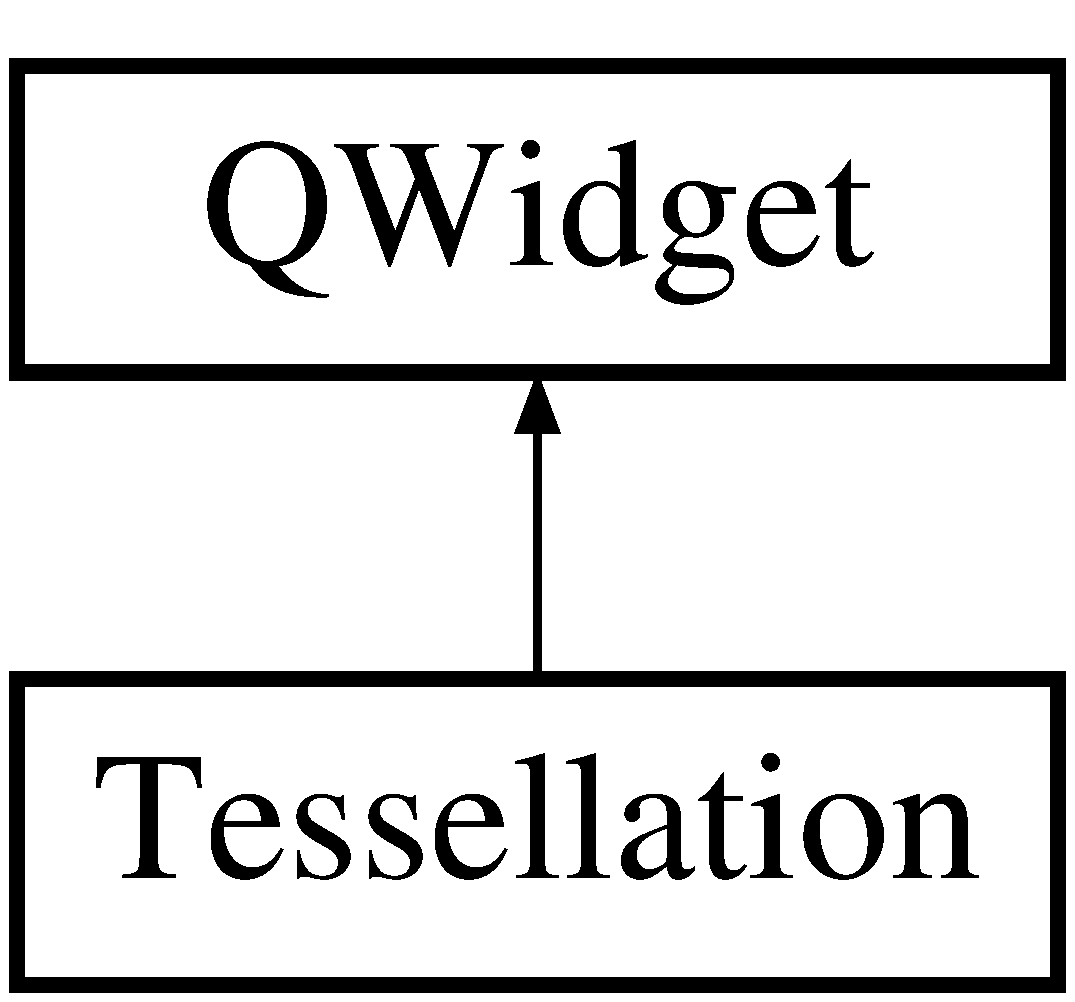
\includegraphics[height=2.000000cm]{class_tessellation}
\end{center}
\end{figure}
\subsection*{Public Member Functions}
\begin{DoxyCompactItemize}
\item 
\hyperlink{class_tessellation_a3d77f5ad7aa19936ab47b43b7251526f}{Tessellation} (Q\+Widget $\ast$parent=0)
\begin{DoxyCompactList}\small\item\em Constructor. Creates a tesselation like this\+:  \end{DoxyCompactList}\item 
int \hyperlink{class_tessellation_a7d911890db50eb39146c1ec2d771a7dd}{get\+Rotation} ()
\begin{DoxyCompactList}\small\item\em Getter for the rotation. \end{DoxyCompactList}\item 
int \hyperlink{class_tessellation_a9280b338ed41af0ec33e81391e76f82a}{get\+Width} ()
\begin{DoxyCompactList}\small\item\em Getter for the tesseltation width. \end{DoxyCompactList}\item 
int \hyperlink{class_tessellation_a5fbfd2325a4ba0b7d4e66ce98e474c56}{get\+Height} ()
\begin{DoxyCompactList}\small\item\em Getter for the tesseltation height. \end{DoxyCompactList}\item 
void \hyperlink{class_tessellation_a4ee5bac93c53b25ff1d4ec8a43fdad64}{set\+Rotation} (int r)
\begin{DoxyCompactList}\small\item\em Setter for the tesselation rotation. \end{DoxyCompactList}\item 
void \hyperlink{class_tessellation_aa035a163e76a1616c58d20938b2853aa}{set\+Width} (int w)
\begin{DoxyCompactList}\small\item\em Setter for the tesselation width. \end{DoxyCompactList}\item 
void \hyperlink{class_tessellation_a57273ef613b239b6e16ea97085d2f4df}{set\+Height} (int h)
\begin{DoxyCompactList}\small\item\em Setter for the tesselation height. \end{DoxyCompactList}\end{DoxyCompactItemize}
\subsection*{Protected Member Functions}
\begin{DoxyCompactItemize}
\item 
\hypertarget{class_tessellation_aed2d64951d5d8b7e4fefde70c072b7c1}{}void \hyperlink{class_tessellation_aed2d64951d5d8b7e4fefde70c072b7c1}{paint\+Event} (Q\+Paint\+Event $\ast$)\label{class_tessellation_aed2d64951d5d8b7e4fefde70c072b7c1}

\begin{DoxyCompactList}\small\item\em Paints a tessellation in the window every time that a paint event occurs. \end{DoxyCompactList}\end{DoxyCompactItemize}
\subsection*{Private Attributes}
\begin{DoxyCompactItemize}
\item 
int \hyperlink{class_tessellation_ac09f5100d6f72ad8c4d4ff52268434ca}{rotation}
\item 
int \hyperlink{class_tessellation_a943c56fd0f2e174add80b3bbeb11e74b}{width}
\item 
int \hyperlink{class_tessellation_a94b9f62e66d1b4e967483a7aea75b830}{height}
\end{DoxyCompactItemize}


\subsection{Detailed Description}
A class to create tessellations. 

\subsection{Constructor \& Destructor Documentation}
\hypertarget{class_tessellation_a3d77f5ad7aa19936ab47b43b7251526f}{}\index{Tessellation@{Tessellation}!Tessellation@{Tessellation}}
\index{Tessellation@{Tessellation}!Tessellation@{Tessellation}}
\subsubsection[{Tessellation}]{\setlength{\rightskip}{0pt plus 5cm}Tessellation\+::\+Tessellation (
\begin{DoxyParamCaption}
\item[{Q\+Widget $\ast$}]{parent = {\ttfamily 0}}
\end{DoxyParamCaption}
)\hspace{0.3cm}{\ttfamily [explicit]}}\label{class_tessellation_a3d77f5ad7aa19936ab47b43b7251526f}


Constructor. Creates a tesselation like this\+:  


\begin{DoxyParams}{Parameters}
{\em parent} & parent of this tesselation, you should pass a reference to the window where this tesselation \textquotesingle{}lives\textquotesingle{}. \\
\hline
\end{DoxyParams}


\subsection{Member Function Documentation}
\hypertarget{class_tessellation_a5fbfd2325a4ba0b7d4e66ce98e474c56}{}\index{Tessellation@{Tessellation}!get\+Height@{get\+Height}}
\index{get\+Height@{get\+Height}!Tessellation@{Tessellation}}
\subsubsection[{get\+Height}]{\setlength{\rightskip}{0pt plus 5cm}int Tessellation\+::get\+Height (
\begin{DoxyParamCaption}
{}
\end{DoxyParamCaption}
)}\label{class_tessellation_a5fbfd2325a4ba0b7d4e66ce98e474c56}


Getter for the tesseltation height. 

\begin{DoxyReturn}{Returns}
tesselation height 
\end{DoxyReturn}
\hypertarget{class_tessellation_a7d911890db50eb39146c1ec2d771a7dd}{}\index{Tessellation@{Tessellation}!get\+Rotation@{get\+Rotation}}
\index{get\+Rotation@{get\+Rotation}!Tessellation@{Tessellation}}
\subsubsection[{get\+Rotation}]{\setlength{\rightskip}{0pt plus 5cm}int Tessellation\+::get\+Rotation (
\begin{DoxyParamCaption}
{}
\end{DoxyParamCaption}
)}\label{class_tessellation_a7d911890db50eb39146c1ec2d771a7dd}


Getter for the rotation. 

\begin{DoxyReturn}{Returns}
The rotation 
\end{DoxyReturn}
\hypertarget{class_tessellation_a9280b338ed41af0ec33e81391e76f82a}{}\index{Tessellation@{Tessellation}!get\+Width@{get\+Width}}
\index{get\+Width@{get\+Width}!Tessellation@{Tessellation}}
\subsubsection[{get\+Width}]{\setlength{\rightskip}{0pt plus 5cm}int Tessellation\+::get\+Width (
\begin{DoxyParamCaption}
{}
\end{DoxyParamCaption}
)}\label{class_tessellation_a9280b338ed41af0ec33e81391e76f82a}


Getter for the tesseltation width. 

\begin{DoxyReturn}{Returns}
tesselation width 
\end{DoxyReturn}
\hypertarget{class_tessellation_a57273ef613b239b6e16ea97085d2f4df}{}\index{Tessellation@{Tessellation}!set\+Height@{set\+Height}}
\index{set\+Height@{set\+Height}!Tessellation@{Tessellation}}
\subsubsection[{set\+Height}]{\setlength{\rightskip}{0pt plus 5cm}void Tessellation\+::set\+Height (
\begin{DoxyParamCaption}
\item[{int}]{h}
\end{DoxyParamCaption}
)}\label{class_tessellation_a57273ef613b239b6e16ea97085d2f4df}


Setter for the tesselation height. 


\begin{DoxyParams}{Parameters}
{\em h} & tessellation height \\
\hline
\end{DoxyParams}
\hypertarget{class_tessellation_a4ee5bac93c53b25ff1d4ec8a43fdad64}{}\index{Tessellation@{Tessellation}!set\+Rotation@{set\+Rotation}}
\index{set\+Rotation@{set\+Rotation}!Tessellation@{Tessellation}}
\subsubsection[{set\+Rotation}]{\setlength{\rightskip}{0pt plus 5cm}void Tessellation\+::set\+Rotation (
\begin{DoxyParamCaption}
\item[{int}]{r}
\end{DoxyParamCaption}
)}\label{class_tessellation_a4ee5bac93c53b25ff1d4ec8a43fdad64}


Setter for the tesselation rotation. 


\begin{DoxyParams}{Parameters}
{\em r} & tessellation rotation \\
\hline
\end{DoxyParams}
\hypertarget{class_tessellation_aa035a163e76a1616c58d20938b2853aa}{}\index{Tessellation@{Tessellation}!set\+Width@{set\+Width}}
\index{set\+Width@{set\+Width}!Tessellation@{Tessellation}}
\subsubsection[{set\+Width}]{\setlength{\rightskip}{0pt plus 5cm}void Tessellation\+::set\+Width (
\begin{DoxyParamCaption}
\item[{int}]{w}
\end{DoxyParamCaption}
)}\label{class_tessellation_aa035a163e76a1616c58d20938b2853aa}


Setter for the tesselation width. 


\begin{DoxyParams}{Parameters}
{\em w} & tessellation width \\
\hline
\end{DoxyParams}


\subsection{Member Data Documentation}
\hypertarget{class_tessellation_a94b9f62e66d1b4e967483a7aea75b830}{}\index{Tessellation@{Tessellation}!height@{height}}
\index{height@{height}!Tessellation@{Tessellation}}
\subsubsection[{height}]{\setlength{\rightskip}{0pt plus 5cm}int Tessellation\+::height\hspace{0.3cm}{\ttfamily [private]}}\label{class_tessellation_a94b9f62e66d1b4e967483a7aea75b830}
tesselation height / altura del mosaico \hypertarget{class_tessellation_ac09f5100d6f72ad8c4d4ff52268434ca}{}\index{Tessellation@{Tessellation}!rotation@{rotation}}
\index{rotation@{rotation}!Tessellation@{Tessellation}}
\subsubsection[{rotation}]{\setlength{\rightskip}{0pt plus 5cm}int Tessellation\+::rotation\hspace{0.3cm}{\ttfamily [private]}}\label{class_tessellation_ac09f5100d6f72ad8c4d4ff52268434ca}
tesselation rotation / rotacion del mosaico \hypertarget{class_tessellation_a943c56fd0f2e174add80b3bbeb11e74b}{}\index{Tessellation@{Tessellation}!width@{width}}
\index{width@{width}!Tessellation@{Tessellation}}
\subsubsection[{width}]{\setlength{\rightskip}{0pt plus 5cm}int Tessellation\+::width\hspace{0.3cm}{\ttfamily [private]}}\label{class_tessellation_a943c56fd0f2e174add80b3bbeb11e74b}
tesselation width / ancho del mosaico 

The documentation for this class was generated from the following files\+:\begin{DoxyCompactItemize}
\item 
tessellation.\+h\item 
tessellation.\+cpp\end{DoxyCompactItemize}

%--- End generated contents ---

% Index
\backmatter
\newpage
\phantomsection
\clearemptydoublepage
\addcontentsline{toc}{chapter}{Index}
\printindex

\end{document}
